\documentclass[tikz,border=8pt]{standalone}
\usepackage[T1]{fontenc}
\usepackage[utf8]{inputenc}
\usepackage{lmodern}
\usepackage{xcolor}
\usetikzlibrary{arrows.meta,positioning}

\definecolor{astblue}{HTML}{DCEEFF}
\definecolor{astgreen}{HTML}{DFF5E1}
\definecolor{astyellow}{HTML}{FFF3CC}
\definecolor{astpink}{HTML}{FBE1EA}
\definecolor{astgray}{HTML}{F4F4F4}
\definecolor{astline}{HTML}{5A6B7A}

\tikzset{
  box/.style={
    draw=astline,
    rounded corners=3pt,
    thick,
    align=left,
    font=\sffamily\small,
    inner sep=6pt
  },
  title/.style={
    font=\sffamily\bfseries\Large,
    text=black
  },
  arrow/.style={
    -{Latex[length=3mm,width=2mm]},
    thick,
    draw=astline
  },
  note/.style={
    font=\sffamily\footnotesize,
    text=black!75,
    align=left
  }
}

\begin{document}
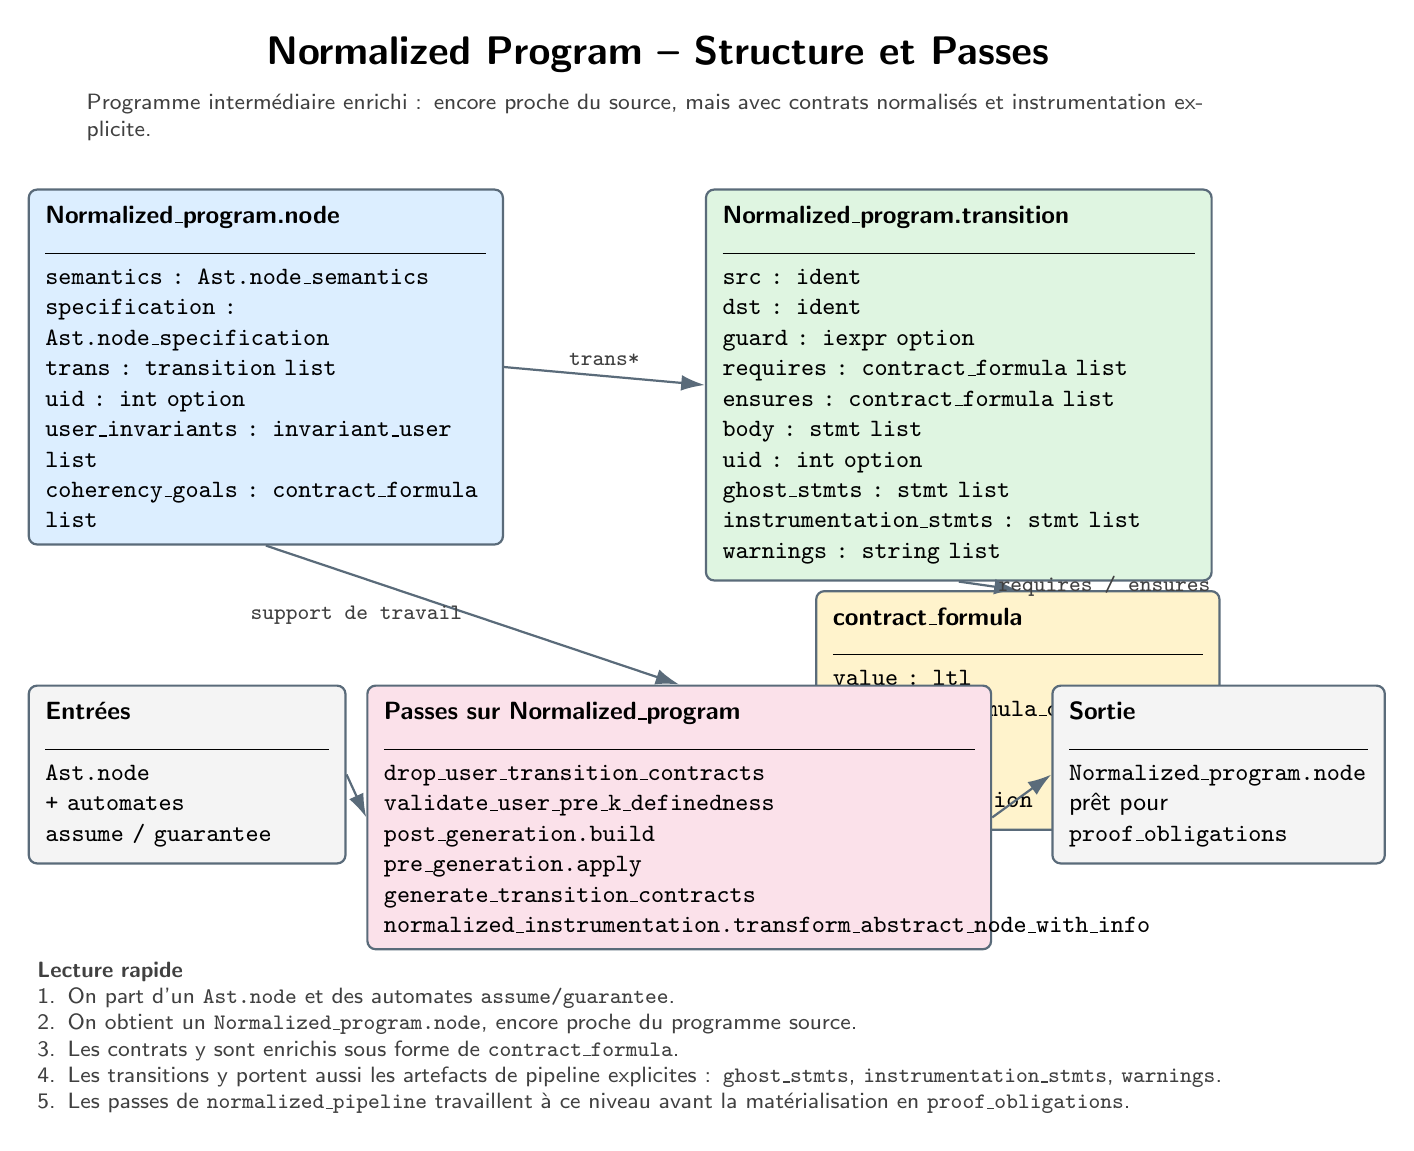
\begin{tikzpicture}[x=1cm,y=1cm]

\node[title] at (8.0, 12.2) {Normalized Program -- Structure et Passes};
\node[note, text width=14.5cm] at (8.0, 11.4)
  {Programme intermédiaire enrichi : encore proche du source, mais avec contrats normalisés et instrumentation explicite.};

\node[box, fill=astblue, text width=5.6cm, anchor=north west] (node) at (0.0, 10.5) {
  \textbf{Normalized\_program.node}\\
  \rule{\linewidth}{0.4pt}\\
  \texttt{semantics : Ast.node\_semantics}\\
  \texttt{specification : Ast.node\_specification}\\
  \texttt{trans : transition list}\\
  \texttt{uid : int option}\\
  \texttt{user\_invariants : invariant\_user list}\\
  \texttt{coherency\_goals : contract\_formula list}
};

\node[box, fill=astgreen, text width=6.0cm, anchor=north west] (transition) at (8.6, 10.5) {
  \textbf{Normalized\_program.transition}\\
  \rule{\linewidth}{0.4pt}\\
  \texttt{src : ident}\\
  \texttt{dst : ident}\\
  \texttt{guard : iexpr option}\\
  \texttt{requires : contract\_formula list}\\
  \texttt{ensures : contract\_formula list}\\
  \texttt{body : stmt list}\\
  \texttt{uid : int option}\\
  \texttt{ghost\_stmts : stmt list}\\
  \texttt{instrumentation\_stmts : stmt list}\\
  \texttt{warnings : string list}
};

\node[box, fill=astyellow, text width=4.7cm, anchor=north west] (formula) at (10.0, 5.4) {
  \textbf{contract\_formula}\\
  \rule{\linewidth}{0.4pt}\\
  \texttt{value : ltl}\\
  \texttt{origin : Formula\_origin.t option}\\
  \texttt{oid : int}\\
  \texttt{loc : loc option}
};

\node[box, fill=astgray, text width=3.6cm, anchor=north west] (input) at (0.0, 4.2) {
  \textbf{Entrées}\\
  \rule{\linewidth}{0.4pt}\\
  \texttt{Ast.node}\\
  \texttt{+ automates}\\
  \texttt{assume / guarantee}
};

\node[box, fill=astpink, text width=7.5cm, anchor=north west] (pipeline) at (4.3, 4.2) {
  \textbf{Passes sur Normalized\_program}\\
  \rule{\linewidth}{0.4pt}\\
  \texttt{drop\_user\_transition\_contracts}\\
  \texttt{validate\_user\_pre\_k\_definedness}\\
  \texttt{post\_generation.build}\\
  \texttt{pre\_generation.apply}\\
  \texttt{generate\_transition\_contracts}\\
  \texttt{normalized\_instrumentation.transform\_abstract\_node\_with\_info}
};

\node[box, fill=astgray, text width=3.8cm, anchor=north west] (output) at (13.0, 4.2) {
  \textbf{Sortie}\\
  \rule{\linewidth}{0.4pt}\\
  \texttt{Normalized\_program.node}\\
  prêt pour\\
  \texttt{proof\_obligations}
};

\node[note, text width=16.3cm, anchor=north west] (legend) at (0.0, 0.8) {
  \textbf{Lecture rapide}\\
  1. On part d'un \texttt{Ast.node} et des automates \texttt{assume/guarantee}.\\
  2. On obtient un \texttt{Normalized\_program.node}, encore proche du programme source.\\
  3. Les contrats y sont enrichis sous forme de \texttt{contract\_formula}.\\
  4. Les transitions y portent aussi les artefacts de pipeline explicites : \texttt{ghost\_stmts}, \texttt{instrumentation\_stmts}, \texttt{warnings}.\\
  5. Les passes de \texttt{normalized\_pipeline} travaillent à ce niveau avant la matérialisation en \texttt{proof\_obligations}.
};

\draw[arrow] (node.east) -- node[midway, above, note] {\texttt{trans*}} (transition.west);
\draw[arrow] (transition.south) -- node[midway, right, note] {\texttt{requires / ensures}} (formula.north);
\draw[arrow] (input.east) -- (pipeline.west);
\draw[arrow] (pipeline.east) -- (output.west);
\draw[arrow] (node.south) -- node[midway, left, note] {\texttt{support de travail}} (pipeline.north);

\end{tikzpicture}
\end{document}
